% Dokumentklassen sættes til memoir.
% Manual: http://ctan.org/tex-archive/macros/latex/contrib/memoir/memman.pdf
\documentclass[a4paper,11pt,twoside,openright,article]{memoir}
\setlrmarginsandblock{*}{2.5cm}{0.75} % højre og venstre 
\setulmarginsandblock{3cm}{*}{1.2} % top og bund 
\checkandfixthelayout[nearest] % specifikt valg af højde algoritme
 
% Danske udtryk (fx figur og tabel) samt dansk orddeling og fonte med
% danske tegn. Hvis LaTeX brokker sig over æ, ø og å skal du udskifte
% "utf8" med "latin1" eller "applemac". 
\usepackage[utf8]{inputenc}
\usepackage[danish]{babel}
\usepackage[T1]{fontenc}
\usepackage{mflogo}

%sexy pdf'er
%\usepackage[export]{adjustbox}
\usepackage{pdfpages}
\usepackage{pdflscape}

%Kompakte lister
\usepackage{paralist}
 
% Matematisk udtryk, fede symboler, theoremer og fancy ting (fx kædebrøker)
\usepackage{amsmath,amssymb}
\usepackage{bm}
\usepackage{amsthm}
\usepackage{mathtools}
\parindent=0pt 

% Fancy ting med enheder og datatabeller. Læs manualen til pakken
% Manual: http://www.ctan.org/tex-archive/macros/latex/contrib/siunitx/siunitx.pdf
\usepackage{siunitx}
 
%Fancy headers, 
%Manual: https://www.sharelatex.com/learn/Headers_and_footers
\let\footruleskip\undefined
\usepackage{fancyhdr}
\pagestyle{fancy}

 
% Indsættelse af grafik. og man kan rotere tekst in line
\usepackage{graphicx} 
\usepackage{fix-cm} 
\usepackage{soul}
\sodef\an{}{0.13em}{0em}{0em} \sodef\ann{}{0.13em}{0.5em}{0em}
 
%Fancy tabeller.
%\usepackage[table]{xcolor}
\usepackage{multirow}
\usepackage{rotating} %sidewaystables!
\usepackage{longtable} %tables spanning multible pages.
\usepackage{tablefootnote} %for at indstætte fornoter i tabeller.
\usepackage{hhline} %Fixer farvede felter
\usepackage{ltxtable} %Longtabular X
\usepackage{tabularx} %Med dynamisk bredte

%URL fodnoter
\usepackage{url}

% Reaktionsskemaer. Læs manualen for at se eksempler.
% Manual: http://www.ctan.org/tex-archive/macros/latex/contrib/mhchem/mhchem.pdf
\usepackage[version=3]{mhchem}

%Lav chapter clickable og fjern border
\usepackage{hyperref}
\hypersetup{
    colorlinks,
    citecolor=black,
    filecolor=black,
    linkcolor=black,
    urlcolor=black
}

%Table of contents settings
\setsecnumdepth{subsection} % organisational level that receives a numbers
\settocdepth{subsection}   % print table of  for level 3

%Til programkode
\usepackage{listings}
\usepackage{color}

\definecolor{dkgreen}{rgb}{0,0.6,0}
\definecolor{gray}{rgb}{0.5,0.5,0.5}
\definecolor{mauve}{rgb}{0.58,0,0.82}
 
\lstset{ 
  language=C++,                % the language of the code
  basicstyle=\footnotesize,           % the size of the fonts that are used for the code
  numbers=left,                   % where to put the line-numbers
  numberstyle=\tiny\color{gray},  % the style that is used for the line-numbers
  stepnumber=1,                   % the step between two line-numbers. If it's 1, each line 
                                  % will be numbered
  numbersep=5pt,                  % how far the line-numbers are from the code
  backgroundcolor=\color{white},      % choose the background color. You must add \usepackage{color}
  showspaces=false,               % show spaces adding particular underscores
  showstringspaces=false,         % underline spaces within strings
  showtabs=false,                 % show tabs within strings adding particular underscores
  frame=single,                   % adds a frame around the code
  rulecolor=\color{black},        % if not set, the frame-color may be changed on line-breaks within not-black text (e.g. commens (green here))
  tabsize=2,                      % sets default tabsize to 2 spaces
  captionpos=b,                   % sets the caption-position to bottom
  breaklines=true,                % sets automatic line breaking
  breakatwhitespace=false,        % sets if automatic breaks should only happen at whitespace
  title=\lstname,                   % show the filename of files included with \lstinputlisting;
                                  % also try caption instead of title
  keywordstyle=\color{blue},          % keyword style
  commentstyle=\color{dkgreen},       % comment style
  stringstyle=\color{mauve},         % string literal style
  escapeinside={\%*}{*)},            % if you want to add LaTeX within your code
  morekeywords={*,...},               % if you want to add more keywords to the set
  rangeprefix=//----------,			%Used for sexy code includes
  rangesuffix=----------,			%---||---
  includerangemarker=false,			%---||---
  literate=
  {á}{{\'a}}1 {é}{{\'e}}1 {í}{{\'i}}1 {ó}{{\'o}}1 {ú}{{\'u}}1
  {Á}{{\'A}}1 {É}{{\'E}}1 {Í}{{\'I}}1 {Ó}{{\'O}}1 {Ú}{{\'U}}1
  {à}{{\`a}}1 {è}{{\`e}}1 {ì}{{\`i}}1 {ò}{{\`o}}1 {ù}{{\`u}}1
  {À}{{\`A}}1 {È}{{\'E}}1 {Ì}{{\`I}}1 {Ò}{{\`O}}1 {Ù}{{\`U}}1
  {ä}{{\"a}}1 {ë}{{\"e}}1 {ï}{{\"i}}1 {ö}{{\"o}}1 {ü}{{\"u}}1
  {Ä}{{\"A}}1 {Ë}{{\"E}}1 {Ï}{{\"I}}1 {Ö}{{\"O}}1 {Ü}{{\"U}}1
  {â}{{\^a}}1 {ê}{{\^e}}1 {î}{{\^i}}1 {ô}{{\^o}}1 {û}{{\^u}}1
  {Â}{{\^A}}1 {Ê}{{\^E}}1 {Î}{{\^I}}1 {Ô}{{\^O}}1 {Û}{{\^U}}1
  {œ}{{\oe}}1 {Œ}{{\OE}}1 {æ}{{\ae}}1 {Æ}{{\AE}}1 {ß}{{\ss}}1
  {ç}{{\c c}}1 {Ç}{{\c C}}1 {ø}{{\o}}1 {å}{{\r a}}1 {Å}{{\r A}}1
  {€}{{\EUR}}1 {£}{{\pounds}}1
}

%Til at udregne forskel mellem sider, brug \pagedifference{A}{B} mellem to labels A og B.
\usepackage{refcount}
\newcommand{\pagedifference}[2]{%
  \number\numexpr\getpagerefnumber{#2}-\getpagerefnumber{#1}\relax}
 
%Til at lave referencer med:
\usepackage{cite}

%Til at lave eksterne \ref til \labels
\usepackage{xr}

%Til at lave \Beam (DC symbol)
\usepackage{marvosym}

%Forsøg på nice lister i tabeller
\usepackage[shortlabels]{enumitem}

\newenvironment{packed_enum}{
\begin{enumerate}[1., topsep=0pt, nosep, partopsep=0pt, itemsep=0pt, parsep=0pt]
}{\end{enumerate}}

\newenvironment{packed_item}{
\begin{itemize}[•, topsep=0pt, nosep, partopsep=0pt, itemsep=0pt, parsep=0pt]
}{\end{itemize}}

%Lækker kommando til at skrive I2C flot uden at bruge \textsuperscript hver gang:
\newcommand*{\IIC}{\texorpdfstring{I\textsuperscript{2}C }{I2C }}

%Lorem ipsum
\usepackage{lipsum}


\usepackage{longtable}
\usepackage{array} % for extrarowheight

%Juicy columntypes - http://tex.stackexchange.com/questions/12703/how-to-create-fixed-width-table-columns-with-text-raggedright-centered-raggedlef
\newcolumntype{L}[1]{>{\raggedright\let\newline\\\arraybackslash\hspace{0pt}}p{#1}}
\newcolumntype{C}[1]{>{\centering\let\newline\\\arraybackslash\hspace{0pt}}p{#1}}
\newcolumntype{R}[1]{>{\raggedleft\let\newline\\\arraybackslash\hspace{0pt}}p{#1}}
\newcolumntype{Z}{>{\raggedright\arraybackslash}X}

%Dejlig kommando til at få nye kapitler på højre side
\newcommand*\cleartorightpage{%
	\clearpage
 	\checkoddpage
	\ifoddpage
  		%do nothing
	\else
		\thispagestyle{empty}
		\mbox{}
 		\clearpage
	\fi
}


%Hacky løsning til at ordne indholdsfortegnelsen.. Why memoir class.. WHY??!
\renewcommand*{\cftdotsep}{1}
\setpnumwidth{3em}
\setrmarg{4em}

%Bugfix til Longtables
\makeatletter
\def\LT@start{%
  \let\LT@start\endgraf
  \endgraf\penalty\z@\vskip\LTpre
  \dimen@\pagetotal
  \advance\dimen@ \ht\ifvoid\LT@firsthead\LT@head\else\LT@firsthead\fi
  \advance\dimen@ \dp\ifvoid\LT@firsthead\LT@head\else\LT@firsthead\fi
  \advance\dimen@ \ht\LT@foot
  \edef\restore@vbadness{\vbadness\the\vbadness\relax}% (added)
  \vbadness=\@M % (added)
  \dimen@ii\vfuzz
  \vfuzz\maxdimen
    \setbox\tw@\copy\z@
    \setbox\tw@\vsplit\tw@ to \ht\@arstrutbox
    \setbox\tw@\vbox{\unvbox\tw@}%
  \vfuzz\dimen@ii
  \restore@vbadness % (added)
  \advance\dimen@ \ht
        \ifdim\ht\@arstrutbox>\ht\tw@\@arstrutbox\else\tw@\fi
  \advance\dimen@\dp
        \ifdim\dp\@arstrutbox>\dp\tw@\@arstrutbox\else\tw@\fi
  \advance\dimen@ -\pagegoal
  \ifdim \dimen@>\z@\vfil\break\fi
      \global\@colroom\@colht
  \ifvoid\LT@foot\else
    \advance\vsize-\ht\LT@foot
    \global\advance\@colroom-\ht\LT@foot
    \dimen@\pagegoal\advance\dimen@-\ht\LT@foot\pagegoal\dimen@
    \maxdepth\z@
  \fi
  \ifvoid\LT@firsthead\copy\LT@head\else\box\LT@firsthead\fi\nobreak
  \output{\LT@output}%
}
\makeatother

\title{EMC Rapport \\ AU2 \\ \textit{Den intelligente bil}\\ Gruppe 1}
\author{4. Semesterprojekt E4PRJ4 \\ Ingeniørhøjskolen, Aarhus Universitet\\ Vejleder: Arne Justesen}
\date{\today}

\begin{document}
\fancyhf{} %Clear all header/footers
\frontmatter
\maketitle
\vfill

\begin{table} [h]
	\centering
	\begin{tabular}{|l|r|l|}
	\hline 
	\textbf{Navn} 				& \textbf{Studienummer} & \textbf{Underskrift~~~~~~~~~~~~~~~~~~~~} 	\\ \hline
	Kristian Thomsen 			& 201311478 & \\ && 												\\ \hline
	Philip Krogh-Pedersen 		& 201311473 & \\ && 												\\ \hline
	Lasse Barner Sivertsen 		& 201371048 & \\ && 												\\ \hline
	Henrik Bagger Jensen 		& 201304157 & \\ && 												\\ \hline
	Kenn Hedegaard Eskildsen 	& 201370904 & \\ && 												\\ \hline
	Karsten Schou Nielsen 		& 201370045 & \\ && 												\\ \hline
	Jesper Pedersen 			& 201370530 & \\ && 												\\ \hline
	\end{tabular}
\end{table}
\clearpage
\pagestyle{plain}

\tableofcontents

\vfill
%\chapter{Arbejdsopgaver}\label{ch:arbejdsopgaver}
%TODO Ret denne tabel
Under projektarbejdet har arbejdsopgaver været fordelt efter følgende tabel:

\begin{table}[h]
\centering
\begin{tabularx}{\textwidth * 6/7}{Z|l|l|l|l|l|l|l|}
	\cline{2-8}
	~ & \rotatebox{90}{Kristian Thomsen~~} 
	& \rotatebox{90}{Philip Krogh-Pedersen} 
	& \rotatebox{90}{Lasse Barner Sivertsen} 
	& \rotatebox{90}{Henrik Bagger Jensen} 
	& \rotatebox{90}{Kenn Hedegaard Eskildsen} 
	& \rotatebox{90}{Karsten Schou Nielsen} 
	& \rotatebox{90}{Jesper Ellebæk Pedersen}\\ \hline
	\multicolumn{1}{|X|}{Projektformulering} 	& X & X & X & X & X & X & X  \\\hline
	\multicolumn{1}{|X|}{Kravspecifikation} 	& X & X & X & X & X & X & X \\\hline
	\multicolumn{1}{|X|}{Systemarkitektur} 		& X & X & X & X & X & X & X \\\hline
	\multicolumn{1}{|X|}{Protokol GUI} 			&  &  &  &  &  & X &  \\\hline
	\multicolumn{1}{|X|}{Protokol Kamera } 		&  &  &  &  &  & X &  \\\hline
	\multicolumn{1}{|X|}{HW Design og impl. - Bil: Strømforsyning} & X &  &  &  &  &  &  \\\hline
	\multicolumn{1}{|X|}{HW Design og impl. - Bil: Motorstyring} &  &  &  &  &  &  &  X \\\hline
	\multicolumn{1}{|X|}{HW Design og impl. - Bil: Tachometer} &  &  &  &  &  &  & X \\\hline
	\multicolumn{1}{|X|}{SW Design og impl. - Bil: Steering klassen} &  &  &  &  &  &  & X \\\hline
	\multicolumn{1}{|X|}{SW Design og impl. - PC: Software} &  &  &  &  &  & X &  \\\hline
	\multicolumn{1}{|X|}{SW Design og impl. - PC: XboxController klassen} &  &  & X &  &  &  &  \\\hline
	\multicolumn{1}{|X|}{SW Design og impl. - Bil: Kamera software} &  &  &  &  &  & X &  \\\hline
	\multicolumn{1}{|X|}{SW Design og impl. - Bil: Log og Data klasserne} &  & X &  &  &  &  &  \\\hline
	\multicolumn{1}{|X|}{SW Design og impl. - Bil: PcCom og Settings klasserne} &  &  & X &  &  &  &  \\\hline
	\multicolumn{1}{|X|}{SW Design og impl. - Bil: DistanceSensor} &  &  &  &  & X &  &  \\\hline
	\multicolumn{1}{|X|}{SW Design og impl. - Bil: Aks og Pi klasserne} & X &  &  &  &  &  &  \\\hline
	\multicolumn{1}{|X|}{Accepttest} & X & X & X & X & X & X & X  \\\hline
	\multicolumn{1}{|X|}{Rapport} & X & X & X & X & X & X & X \\\hline
	\end{tabularx}
\end{table}

\mainmatter
\pagestyle{fancy}
\fancyhf{} %Clear all header/footers
\fancyhead[RO,LE]{Gruppe 1 - AU2}
\fancyhead[CE,CO]{\nouppercase{\leftmark}}
\fancyhead[LO,RE]{IHA, AU}
\fancyfoot[CO,CE]{\nouppercase{\rightmark}}
\fancyfoot[LE,RO]{\thepage}

\chapter{Projektbeskrivelse}

Svissen svassen

\chapter{Implementerede kredsløb}

De implementerede kredsløb er som nævnt tidligere valgt ud fra at der er tale om store strømme, stejle flanker og støjfølsomhed omkring måling af hastighed. 
I hvert afsnit herunder er det beskrevet hvilke specifikke kredsløb det drejer sig om, hvilke EMC-mæssige problemer der forventes at opstå samt hvad gruppen har gjort for at løse eller formindske disse problemer.

\section{Strømforsyning}
\subsection{Printudlæg}

For at implementere kredsløbet i figur \ref{fig:bil_psu} på side \pageref{fig:bil_psu} er der udarbejdet et PCB layout for strømforsyningen.
Dette kan ses i figur \ref{fig:bil_psu_pcb}. 
Under udlægget af printet er der taget forbehold for at minimere arealet af strømsløjfer, som ligger i forbindelse med den skiftende udgang samt returveje derfra på LM26003. Ydermere er der også forsøgt at give så god elektrisk kontakt som muligt ved hjælp af brede printbaner til de komponenter, som forventes at trække en stor, evt. skiftende, strøm.
Dette kan ses i området omkring 3V udgangen fx, da diode, spole, udgang samt kondensator ligger helt op ad hinanden. 
De kredse, som ligger i forbindelse med tilbagekoblingen til LM26003 ligger på den 'nedre' del af printet for at minimere støjen fra de skarpe flanker på LM26003's udgang (ben 1-3 og 11-13).
Grundet at skolens komponentlager ikke lå inde med keramiske kondensatorer i størrelsen 6.8 $\mu F$ er der i stedet sat 7 parallelkoblede kondensatorer i på hver 1 $\mu F$.

\vfill

\begin{figure}[h]
\centering
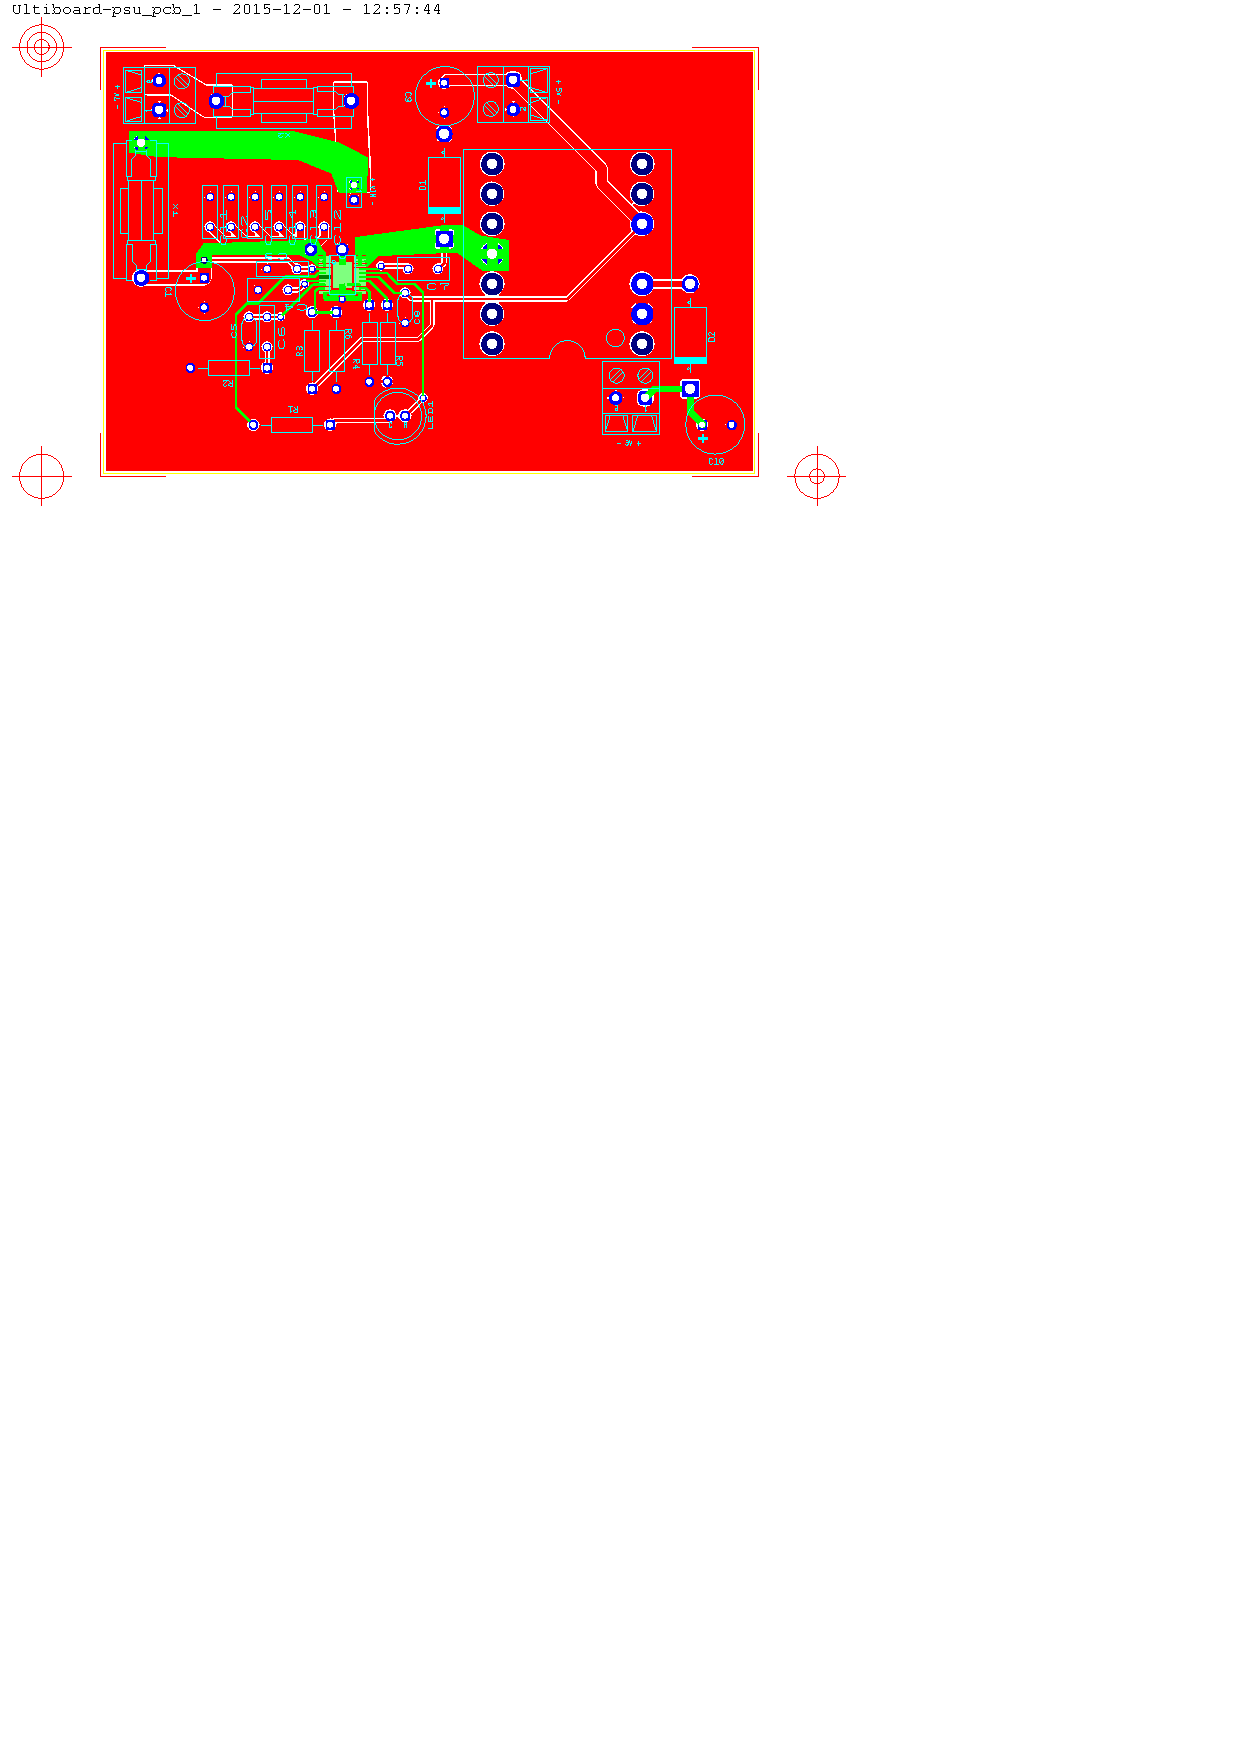
\includegraphics[angle=90,height=\textheight-9cm, clip=true, trim=50 615 234 25]{../fig/diagrammer/bil/psu_pcb_twoside}
\caption{Bilens strømforsyning på PCB}
\label{fig:bil_psu_pcb}
\end{figure}

\clearpage

\subsection{Test}

For at teste strømforsyningen er denne koblet op mod en laboratoriespændingsforsyning indstillet til 7.2V DC.
\section{Tachometer på bil}

Tachometeret består af en TLE4905 \cite{lib:tle4905}
hallswitch, som fungerer ved at detektere magneter rettet i en bestemt retning. Kredsløbet er konstrueret således at hallswitchen trækker signalet til GND, når der detekteres en magnet. Kredsløbet bruger en meget lille strøm, målt til ca. 1.32mA, under tilstedeværelse af en magnet, uden er der målt en strøm på 5 $520\mu A$ . Med en forsyningsspænding på 5V bliver det til en effekt på 6.6mW, hvilket ikke betragtes som nogen EMC-mæssig trussel. Dog er der strømloops i systemet, som på tidspunkter vil være udsat for højfrekvente skift i strøm, hvilket er forsøgt forhindret ved at designe omtalte loops så små som muligt. Grundet det færdige prints størrelse, er det ikke muligt at placere det så tæt som muligt på hjulet som ønsket, hvorfor ledningerne ud til hall-switchen vil være snoede, således der fremkommer en common-mode støj.

\begin{figure}[h]
\centering
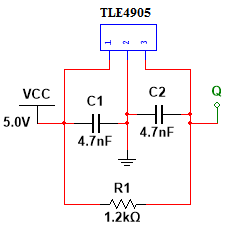
\includegraphics[scale=1]{../fig/billeder/tachometer_multisim.png}
\caption{Design af bilens tachometer i multisim.}
\label{fig:tachometer_multisim}
\end{figure}

Tachometeret er for så vidt ikke være truet af støjoverkobling fra andre kredsløb i systemet, da outputtet ligger fra 0V-5V, og der tælles på logisk LOW, ved Raspberry PI's GPIO. Dvs. at selvom der ligger 1V støj på outputtet, vil det ikke have nogen betydning for tachometerets præcision. Eftersom strømmene i kredsløbet er så små, vil der aldrig kunne induceres en spænding der er tilsvarene, hvilket betyder at der kan ses helt bort fra støjgenerering fra kredsløbet.  Dog er der for god ordens skyld sørget for, at placere kredsløbet så langt fra motorkredsløbet som fysik muligt. 

\clearpage
\section{Motor med tilh. H-bro på bil}

Motorkredsløbet for AU2 vil potentielt være et større EMC-problem, da en højfrekvent og stor strøm løber igennem dele af kredsløbet.
Da motoren drives af et relativt højfrekvent PWM signal, hvis flanker går fra stel til forsyning (7.2V) og der iøvrigt trækkes relativt store strømme. 
Ydermere forventes et spændingspeak når motoren afbrydes ved hver periode, da der løber strøm i spolen og denne strøm ingen steder kan løbe umiddelbart.
Dette giver anledning til højere harmoniske frekvenser af grundfrekvensen i PWM signalet og det vurderes derved at motor agerer som en kraftig støjkilde.

\begin{figure}[h]
\centering
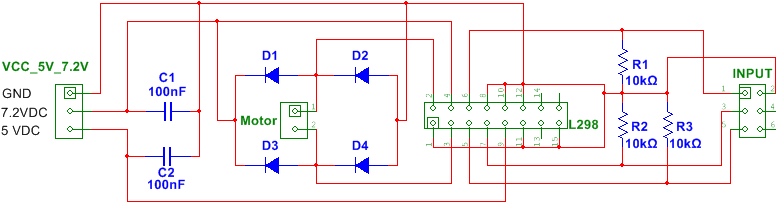
\includegraphics[width=\textwidth]{../fig/billeder/hbro_multisim.png}
\caption{Design af motorens Hbro i Multisim.}
\label{fig:hbro_multisim}
\end{figure}
 
For at modvirke dette er der placeret en kondensator parallelt med motoren, som derved fjerner en stor del af den højfrekvente støj som opstår. 
OBS: Denne kondensator fremgår ikke af figur \ref{fig:hbro_multisim}. 
Dog vil strømmen der tænder og slukker i ledningerne før motoren, kunne give problemer ifm. nærværende ledninger/printbaner. 

\begin{figure}[h]
\centering
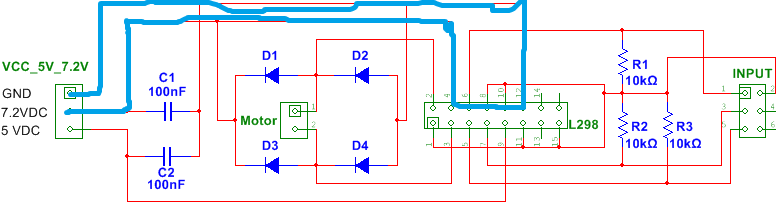
\includegraphics[width=\textwidth]{../fig/billeder/hbro_multisim_loop.png}
\caption{Design af motorens Hbro i Multisim.}
\label{fig:hbro_multisim_loops}
\end{figure}

De strømloops der er i H-broen kan ses på figur \ref{fig:hbro_multisim_loops}. Det blå loop er den strøm der løber fra kondensatoren C1 gennem H-broen til motoren og tilbage via stel. C1 har desuden til formål at reducere støj fra motorkredsløbet på forsyningsnettet.
Det grønne loop er den vej strømmen løber, når enable signalet til H-broen netop er frakoblet og motoren vil forsøge at aflevere energi tilbage til C1. Den forhindrer således spændingspeak fra motoren, men resultatet bliver et strømloop som støjer. Det grønne loop har et tilsvarende strømloop gennem D3 og D2, når DC-motoren kører modsatrettet.
Printet til motorkredsløbet er forsøgt designet således, at de strømloops der er, konstrueres så små som mulige og at banerne med stor risiko for støj er placeret så langt som muligt fra andre baner. Desuden er der placeret et Ground plan, der foruden at forøge stelkapaciteten gør det nemmere for højfrekvente strømme, at finde den returvej med mindst modstand. Printudlægget kan ses på figur \ref{fig:hbro_ultiboard}.
C1 og C2 er placeret på bagsiden af printet under D2, dette kan godt være svært at se grundet farvevalget.

Som en ekstra forsikring mod common-modestøj, kan man med tilledningerne ud til motoren påsætte en ferritkerne omkring, som derved vil fjerne meget af støjen fra den strøm som løber ud til motoren.

\begin{figure}[h]
\centering
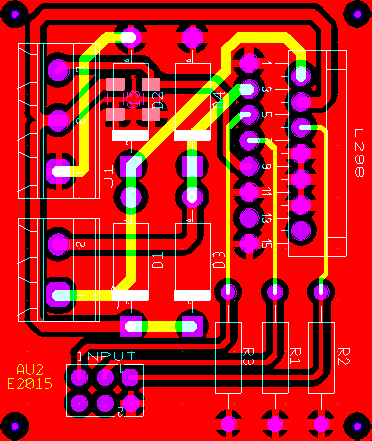
\includegraphics[scale=1]{../fig/billeder/hbro_ultiboard.png}
\caption{Printdesign af motorens Hbro i Ultiboard.}
\label{fig:hbro_ultiboard}
\end{figure}


\renewcommand{\bibname}{Litteraturliste}
\fancyhead[CE,CO]{}
\fancyfoot[CE,CO]{}
\begin{thebibliography}{2}

%SKABELON*** \bibitem{lib:##REF##} ##FIRMANAVN##: \textit{##FORKLARING##}. \\ ##\URL{} ELLER BILAG XXX??##. ##DATO##

\bibitem {lib:MIPICSI-2} Mipi Alliance: \textit{Kamera interface standard}. \\ 
\url{http://mipi.org/specifications/camera-interface}. 2015.

\bibitem {lib:PI2PSU} RASPBERRY PI FOUNDATION: \textit{Anbefalet PSU størrelse}. \\
\url{https://www.raspberrypi.org/help/faqs/#powerReqs}. 2015.

\bibitem {lib:maxsonar} MaxBotix: \textit{I2CXL-MaxSonar-EZ0 datablad}. \\
\url{http://www.maxbotix.com/Ultrasonic_Sensors/MB1202.htm}. 2015.

\bibitem {lib:servo} Corona: \textit{CS238MG Metal Gear Servo datablad}. \\
\url{http://kurser.iha.dk/eit/eit-lab/embeddedStock/Datasheet/CS238MG.pdf}. 2015.

\bibitem {lib:accel} InvenSense: \textit{MPU-6050 accelerometer datablad}. \\
\url{http://www.invensense.com/products/motion-tracking/6-axis/mpu-6050/}. 2015.

\bibitem {lib:tacho} SIEMENS: \textit{TLE4905L Hall Switch til tachometer}. \\
\url{http://www.alldatasheet.com/datasheet-pdf/pdf/45868/SIEMENS/TLE4905L.html}. 2015.

\bibitem {lib:psu_L1core} EPCOS: \textit{ETD 29/16/10 spolekerne og form datablad}. \\
\url{http://en.tdk.eu/inf/80/db/fer_13/etd_29_16_10.pdf}. 2015.

\bibitem {lib:psu_calcs} Kristian Thomsen: \textit{Beregninger for bilens strømforsyning}. \\
Bilag 001. 2015.

\bibitem {lib:analogteknik} Tore Skogberg: \textit{Analogteknik T-005 v1.2}.\\
Bilag 002. 2015.

\bibitem {lib:lm26003} Texas Instruments: \textit{LM26003 datablad}. \\
\url{http://www.ti.com/product/lm26003}. 2015.

\bibitem {lib:vlc-ftp} VLC mediaplayer plugins: \\
\url{ftp://ftp.videolan.org/pub/videolan/vlc/2.0.7/win32/}

\bibitem {lib:qt} Qt creator: \\
\url{http://www.qt.io/ide/}

\bibitem {lib:vlc-qt} vlc-qt-libary: \\
\url{https://vlc-qt.tano.si/}

\bibitem {lib:vlc-using-qt} vlc using qt: \\
\url{http://derekmolloy.ie/custom-video-streaming-player-using-libvlc-and-qt/}

\bibitem {lib:tle4905} Siemens: \textit{TLE4905 datablad}. \\
Bilag 003. 1997-09-1.

\bibitem {lib:qt-bog} C++ GUI programming in Qt: \\
\url{http://www.bogotobogo.com/cplusplus/files/c-gui-programming-with-qt-4-2ndedition.pdf}

\bibitem {lib:motion-on-raspberry} motion on raspberry: \\
\url{http://captain-slow.dk/2013/11/01/install-motion-on-a-raspberry-pi/}

\bibitem {lib:motion-on-raspberry2} motion on raspberry: \\
\url{https://discourse.osmc.tv/t/trying-to-install-motion-missing-libs/5709/9}

\bibitem {lib:camera-driver} uv4l Camera driver: \\
\url{http://www.linux-projects.org/modules/sections/index.php?op=viewarticle&artid=14}

\bibitem {wikiPWM} Wikipedia PWM \\
\url{https://en.wikipedia.org/wiki/Pulse-width_modulation}

\bibitem {L298N_datablad} STMicroelectronics: \textit{L298N datablad} \\
Bilag 004. 2000

\bibitem {wikiHbro} Wikipedia H-bro \\
\url{https://en.wikipedia.org/wiki/H_bridge}

\bibitem{Corona-CS238MG} Corano: \textit{CS238MG}\\
Bilag 005 20??

\end{thebibliography}

\end{document}